\documentclass[oneside]{report}
\usepackage[utf8]{inputenc}
% \usepackage[vietnamese]{babel}
\usepackage[T5]{fontenc}
\usepackage{graphicx}
\usepackage{nameref}
\usepackage{multicol}
\usepackage[vietnamese, main=english]{babel}

% set font, font size and spacing
\usepackage{times}
\usepackage{scrextend}
\changefontsizes{13pt}
\renewcommand{\baselinestretch}{1.3}

% section spacing
\usepackage{titlesec}
\titlespacing*{\section}{0pt}{0.5\baselineskip}{0.2\baselineskip}
\titlespacing*{\subsection}{0pt}{0.4\baselineskip}{0.2\baselineskip}

% setup page layout
\usepackage[a4paper,left=30mm,top=20mm,bottom=25mm,right=20mm,]{geometry}

% Acronyms Auto
\usepackage[nopostdot,toc,acronym,nomain,nonumberlist]{glossaries}
\makeglossaries
\setacronymstyle{long-short}
\loadglsentries[acronym]{FrontMatter/Acronyms}
\setlength{\glsdescwidth}{0.7\linewidth}

% % prevent text overflow
% \usepackage{babel}
% \newcommand\fh{\babelhyphen{hard}}

% Change indent
% \usepackage{indentfirst} % indent also after section titles
\setlength{\parindent}{1cm}
\usepackage{enumitem}
\setlist{leftmargin=1cm}

% paragraph spacing
\setlength{\parskip}{0.5em}

% Change enumerate label
\usepackage{enumitem}

% Page numbering at the center top of page
% \usepackage{fancyhdr} % Custom headers and footers
% \pagestyle{fancyplain} % Makes all pages in the document conform to the custom headers and footers
% \fancyhead[L]{}% Empty left header
% \fancyhead[C]{\thepage} % Page numbering for center header  
% \fancyhead[R]{}% Empty right header
% \fancyfoot[L]{}% Empty left footer
% \fancyfoot[C]{}% Empty center footer
% \fancyfoot[R]{}% Empty left footer

% natbib
% if use natbib, please comment out the cite
\usepackage[sort,numbers]{natbib}
% Citation
% \usepackage{cite}

% Math equation
\usepackage{amssymb}
\usepackage{amsmath}

% Table
\usepackage{multirow}
\usepackage{longtable}
\usepackage{bigstrut}

% Cover
\usepackage{pdfpages}

% Subfigure
\usepackage{caption}
\usepackage{subcaption}

% pstricks fig
\usepackage{epsfig}

% Table of Contents
\usepackage[hidelinks]{hyperref}
% Uncomment if you want leading dot for chapter
\usepackage{tocloft}
\renewcommand{\cftpartleader}{\cftdotfill{\cftdotsep}} % for parts
\renewcommand{\cftchapleader}{\cftdotfill{\cftdotsep}} % for chapters

% table fixed width column
\usepackage{array}
\newcolumntype{L}[1]{>{\raggedright\let\newline\\\arraybackslash\hspace{0pt}}m{#1}}
\newcolumntype{C}[1]{>{\centering\let\newline\\\arraybackslash\hspace{0pt}}m{#1}}
\newcolumntype{R}[1]{>{\raggedleft\let\newline\\\arraybackslash\hspace{0pt}}m{#1}}

\hyphenation{Nan-yang}

\title{GRAPH ATTENTION NETWORKS}
\author{Đoàn Văn Nguyên, Nguyễn Đức Trọng, Nguyễn Trần Đạt}
\date{February 2022}

\begin{document}

% thử tiếng việt
%---------------------------------------------
% Front Matter
%---------------------------------------------

\includepdf[pages=-]{FrontMatter/cover.pdf}
\pagenumbering{roman}
\setcounter{page}{3}
\chapter*{Abstract}
\addcontentsline{toc}{chapter}{Abstract}

Chúng tôi giới thiệu Graph Attention Network (GAT), mô hình mạng nơ-ron mới hoạt động trên dữ liệu dạng đồ thị, sử dụng các lớp tự quan tâm đã đặt mặt nạ để cải thiện những nhược điểm của các phương pháp trước đó dựa trên hỗn hợp đồ thị hoặc các ước lượng của chúng. Bằng cách xếp lớp trong đó các nút có thể quan tâm đến các đặc trưng của lân cận, chúng ta cho phép (ẩn dụ) chỉ định các trọng số khác nhau cho các nút trong một lân cận, mà không cần bất kỳ hoạt động ma trận chi phí (như đảo ngược) hoặc phụ thuộc vào việc biết cấu trúc đồ thị trước.
Theo cách này, chúng tôi giải quyết một số vấn đề chính của các mạng nơ-ron đồ thị dựa trên tần số cùng lúc, và làm cho mô hình của chúng tôi dễ dàng áp dụng cho cả vấn đề dẫn chứng và dẫn điểm. Mô hình GAT của chúng tôi đã cho kết quả ??? trên bốn mô hình kiểm thử transductive và inductive: các tập dữ liệu Cora, Citeseer và Pubmed, cùng với tập dữ liệu tương tác protein-protein (ở đây, test graph bị ẩn trong quá trình học máy).


\vspace{8pt}
\noindent \textit{\textbf{Keywords}: Graph Attention Networks(GAT), transductive, Vietnamese multi-aspect dataset.}


\chapter*{Acknowledgements}
\addcontentsline{toc}{chapter}{Acknowledgements}

Lời đầu tiên, chúng em xin cảm ơn Cô Nguyễn Thị Cẩm Vân và các thầy cô trong lab  Data Science and Knowledge Technology Laboratory at University of Engineering and Technology. Các thầy cô đã luôn giúp đỡ và hướng dẫn chúng em viết ra bài báo này.


% We also want to acknowledge my co-supervisor Assoc.Prof Chng Eng Siong from Nanyang Technological University, Singapore for offering me the internship opportunities at NTU, Singapore and leading me working on diverse exciting projects.

% Furthermore, I am very grateful to my external advisor MSc. Le Hoang Quynh, for insightful comments both in my work and in this thesis, for her support, and for many motivating discussions.

% In addition, we have been very privileged to get to know and to collaborate with many other great collaborators.
% I would like to thank BSc. Nguyen Minh Trang and BSc. Nguyen Duc Canh for inspiring discussion, and for all the fun we have had over the last two years.
% I thank to MSc. Ho Thi Nga and MSc. Vu Thi Ly for continuous support during the time in Singapore.

% Finally, I must express my very profound gratitude to my family for providing me with unfailing support and continuous encouragement throughout my years of study and through the process of researching and writing this thesis.
% This accomplishment would not have been possible without them.

Đồng thời em cũng xin cảm ơn khoa Công nghệ thông tin - Trường Đại học Công nghệ đã tạo điều kiện để cho chúng em có được trải nghiệm thực tế trong môi trường nghiên cứu khoa học và tiếp thu nhiều kiến thức bổ ích.
\chapter*{Declaration}
\addcontentsline{toc}{chapter}{Declaration}
We declare that our work has been composed by ourselves and that the work has not be submitted for any other degree or professional qualification.
We confirm that the work submitted is ou own, except where work which has formed part of jointly-authored publications has been included.
Our contribution and those of the other authors to this work have been explicitly indicated below.
We confirm that appropriate credit has been given within this article where reference has been made to the work of others.

% The model presented in Chapter~\ref{chap:model} and the results presented in Chapter~\ref{chap:result} was previously published in the Proceedings of ACIIDS 2019 as \textit{``Improving Semantic Relation Extraction System with Compositional Dependency Unit on Enriched Shortest Dependency Path''} and NAACL-HTL 2019 as \textit{``A Richer-but-Smarter Shortest Dependency Path with Attentive Augmentation for Relation Extraction''} by myself et al.
% This study was conceived by all of the authors.
% I carried out the main idea(s) and implemented all the model(s) and material(s).

We certify that, to the best of our knowledge, our article does not infringe upon anyone’s copyright nor violate any proprietary rights and that any ideas, techniques, quotations, or any other material from the work of other people included in my thesis, published or otherwise, are fully acknowledged in accordance with the standard referencing practices.
Furthermore, to the extent that we have included copyrighted material, we certify that we have obtained a written permission from the copyright owner(s) to include such material(s) in our work and have fully authorship to improve these materials.

\begin{table}[h]
\begin{tabular}{p{0.7\textwidth}c}
 & Student group \\
 &              \\
 &              \\
 &              \\
 & \textbf{Le Thi Phuong}\\
 & \textbf{Le Minh Binh}\\
 & \textbf{Tran Khanh Hung}\\
 & \textbf{Bui Khanh Huyen}
\end{tabular}
\end{table}

% Show ToC and change title to Table of Contents
\setcounter{secnumdepth}{3}
\renewcommand{\contentsname}{Table of Contents}
\addcontentsline{toc}{chapter}{Table of Contents}
\tableofcontents

% Show Acronyms and add it to ToC
\printglossary[title={Acronyms},type=acronym,style=long]
\clearpage




%--------------------------------------------- 
% Main content
%---------------------------------------------
\pagenumbering{arabic}
\setcounter{page}{1}

\chapter{Giới thiệu}
\label{chap:Giới thiệu}



\section{Nhận Diện Cảm Xúc Trong Hội Thoại (Emotion Recognition in Conversation - ERC)}
\label{sec:Nhận Diện Cảm Xúc Trong Hội Thoại (Emotion Recognition in Conversation - ERC)}

Cảm xúc là một khía cạnh quan trọng trong giao tiếp hàng ngày của con người. 
Vì vậy, trong lĩnh vực xử lí ngôn ngữ tự nhiên, nhận diện cảm xúc là một mảng nghiên cứu càng ngày càng được quan tâm. 

Công nghệ Nhận diện cảm xúc trong hội thoại (ERC) có vai trò xác định trạng thái cảm xúc của người nói trong một cuộc hội thoại. 
ERC có nhiều ứng dụng tiềm năng như hỗ trợ đàm thoại, phân tích cho các thử nghiệm pháp lý và dịch vụ y tế điện tử, v.v.
ERC có rất nhiều tiềm năng khai thác dữ liệu từ các mạng xã hội nổi tiếng trên thế giới như Facebook, Twitter, Youtube, Reddit etc. 
ERC cũng là một thành phần quan trọng để xây dựng các tương tác máy tính tự nhiên như con người và có thể trả lời một cuộc đối thoại có tính cảm xúc.


\section{Multimodal ERC}
\label{sec:Multimodal ERC}

Nhận thấy các nghiên cứu về ERC tập trung vào loại dữ liệu văn bản, *trích bài báo MMGCN* đã đề xuất kết hợp nhiều kiểu dữ liệu khác trong hội thoại (ảnh và tiếng) và ERC, từ đó công bố MMGCN. 

\section{Graph-based Multimodal ERC}
\label{chap:Graph-based Multimodal ERC}

Theo đó, mô hình đồ thị tập trung (Graph Attention Network - GAT) được áp dụng để liên kết các nút trong đồ thị hiệu quả hơn các mô hình trước đây, bằng việc gán trọng số tập trung khác nhau cho từng câu thoại. 

\section{Feature Propagation}
\label{sec:Feature Propagation}

Tuy nhiên, trong nhiều dự án thực tế, các dữ liệu thành phần không phải lúc nào cũng đầy đủ. 
Ví dụ, một câu thoại có thể khuyết thông tin do lỗi dịch thuật hay lỗi của phần mềm chuyển âm thanh thành giọng nói; hay bản ghi âm bị nhiễu do môi trường hay do thiết bị ghi âm.
Đây là một chướng ngại lớn trong việc nhận diện cảm xúc trong hội thoại. 


*trích báo FP* đã đề xuất một phương pháp xử lí dữ liệu bị khuyết, gọi là Lan Truyền Đặc Trưng, sử dụng tối ưu hoá Dirichlet. 
Phương pháp này được hai nhóm tác giả khác kế thừa và phát triển: 

\subsection{Graph Completion Network - GCNET}
GCNET gồm hai mô-đun đồ thị mạng nơ-ron Speaker và Temporal để tách hai loại dữ liệu tương ứng, sau đó được phân loại và tối ưu hoá.

\subsection{Missing Modality Imagination Network - MMIN}
MMIN sử dụng học máy để dự đoán các phần dữ liệu bị khuyết từ dữ liệu có sẵn, trong các điều kiện khác nhau, bằng cách tìm liên hệ giữa các modality với nhau.


\section{Đóng góp}
\label{sec:Đóng góp}

Chúng tôi kết hợp phương pháp lan truyền đặc trưng vào mạng chú ý đồ thị, để xử lí các trường hợp khuyết dữ liệu trong học máy. 
Mô hình này gồm...
\chapter{Dataset Construction}
\label{chap:dataset-construction}


% -------------------------------------------------------------------
% Data Collection
% -------------------------------------------------------------------
\section{Data Collection}
\label{sec:data-collection}

To serve our dedicated approach, we have to handle textual data that are reviews on E-commerce platforms. We choose Scrapy\footnote{\url{https://scrapy.org/}} to crawl the data from online shopping websites including \url{http://www.tiki.vn} and \url{http://www.shopee.vn}. They are two of Vietnam's most common and trusted e-commerce platforms.
We focus on technology and mother \& baby domains since they are the most interested domain in Vietnamese e-commerce.
These raw data are then used as input for Data Annotation step that we will describe in Section~\ref{sec:data-annotation}.

% -------------------------------------------------------------------
% Data Annotation
% -------------------------------------------------------------------
\section{Data Annotation}
\label{sec:data-annotation}
\begin{table}[]
\centering
\resizebox{\linewidth}{!}{
\begin{tabular}{|c|c|>{\raggedright\arraybackslash}m{11 cm}|}
\hline
\textit{\textbf{Domain}}                         & \textit{\textbf{Aspect}} & \multicolumn{1}{c|}{\textit{\textbf{Description}}}                                                                                                                                                                \\ \hline
\multirow{8}{*}{\textbf{Technology}} & Price                    & Cut/ reduce/ slash/ low price considered positive while increase/ put up/ raise/ high price is considered negative.                                            \\ \cline{2-3} 
                               & Service                  & Nice, fast, efficient, enthusiastic support is considered positive while no reply, irresponsibility or carelessly packing is considered negative.                                                                 \\ \cline{2-3} 
                               & Delivery                & The quality, speed and cost of shipping process. If it is fast, carefully shipped and the cost is low, it is considered positive, otherwise is negative.                                                          \\ \cline{2-3} 
                               & Performance              & Fast processing speed is considered positive while lag or latency in the middle of an app or apps shut down unexpectedly is considered negative.                      \\ \cline{2-3} 
                               & Hardware                 & The quality of the hardware of the device including display, chip, battery, cameras, storage, RAM, etc.                                                                                                           \\ \cline{2-3} 
                               & Authenticity             & Genuinely produced product is considered positive while fake, imitation is consider negative.                                                                                                                      \\ \cline{2-3} 
                               & Accessories              & Fully provided, good quality accessories are considered positive; low quality or missed are considered negative.                                                            \\ \cline{2-3} 
                               & Appearance               & Product with nice design, nice color, luxury, etc. are considered positive, product with scratches, awful design is consider negative.                                                                             \\ \hline
\multirow{6}{*}{\textbf{Mother \& Baby}}     & Price                    & Cut/ reduce/ slash/ low price considered positive while increase/ put up/ raise/ high price is considered negative.                                            \\ \cline{2-3} 
                               & Service                  & Nice, fast, efficient, enthusiastic support  is considered positive while no reply, irresponsibility or carelessly packing is considered negative.                                                                 \\ \cline{2-3} 
                               & Delivery               & The quality, speed and cost of shipping process. If it is fast, carefully shipped and the cost is low, it is considered positive, otherwise negative.                                                             \\ \cline{2-3} 
                               & Safety                   & Product having obvious expiration date and has not expired, safe to use is considered positive, while product that is expired or causes allergy, rashes is considered negative. \\ \cline{2-3} 
                               & Quality                  & Customer experience on the product: the softness, absorbency of diapers, the taste and smell of milk, etc.                                                                                                        \\ \cline{2-3} 
                               & Authenticity             & Genuinely produced product is considered positive while fake, imitation is consider negative.                                                                                                                      \\ \hline
\end{tabular}
}
\caption{Aspect description}
\end{table}

We used Docanno as a tool for data annotation. First of all, we overview the data set collected from crawling process to figure out aspects that were frequently mentioned on users’ reviews. 

After discussion, we extracted aspect terms in the sentences and labeled the sentiment polarities with respect to the aspect terms using Docanno. Table 1 illustrates how we handle each aspect. For Technology domain, we predefined eight coarse aspect categories: price, service, delivery, performance, hardware, authenticity, accessories, design. For Mother \& Baby, these are: price, service, delivery, safety, quality and authenticity. In each aspect, it is considered negative when there is at least a complaint regarding that aspect, otherwise it is considered negative.

\begin{figure}[h]
	\centering
	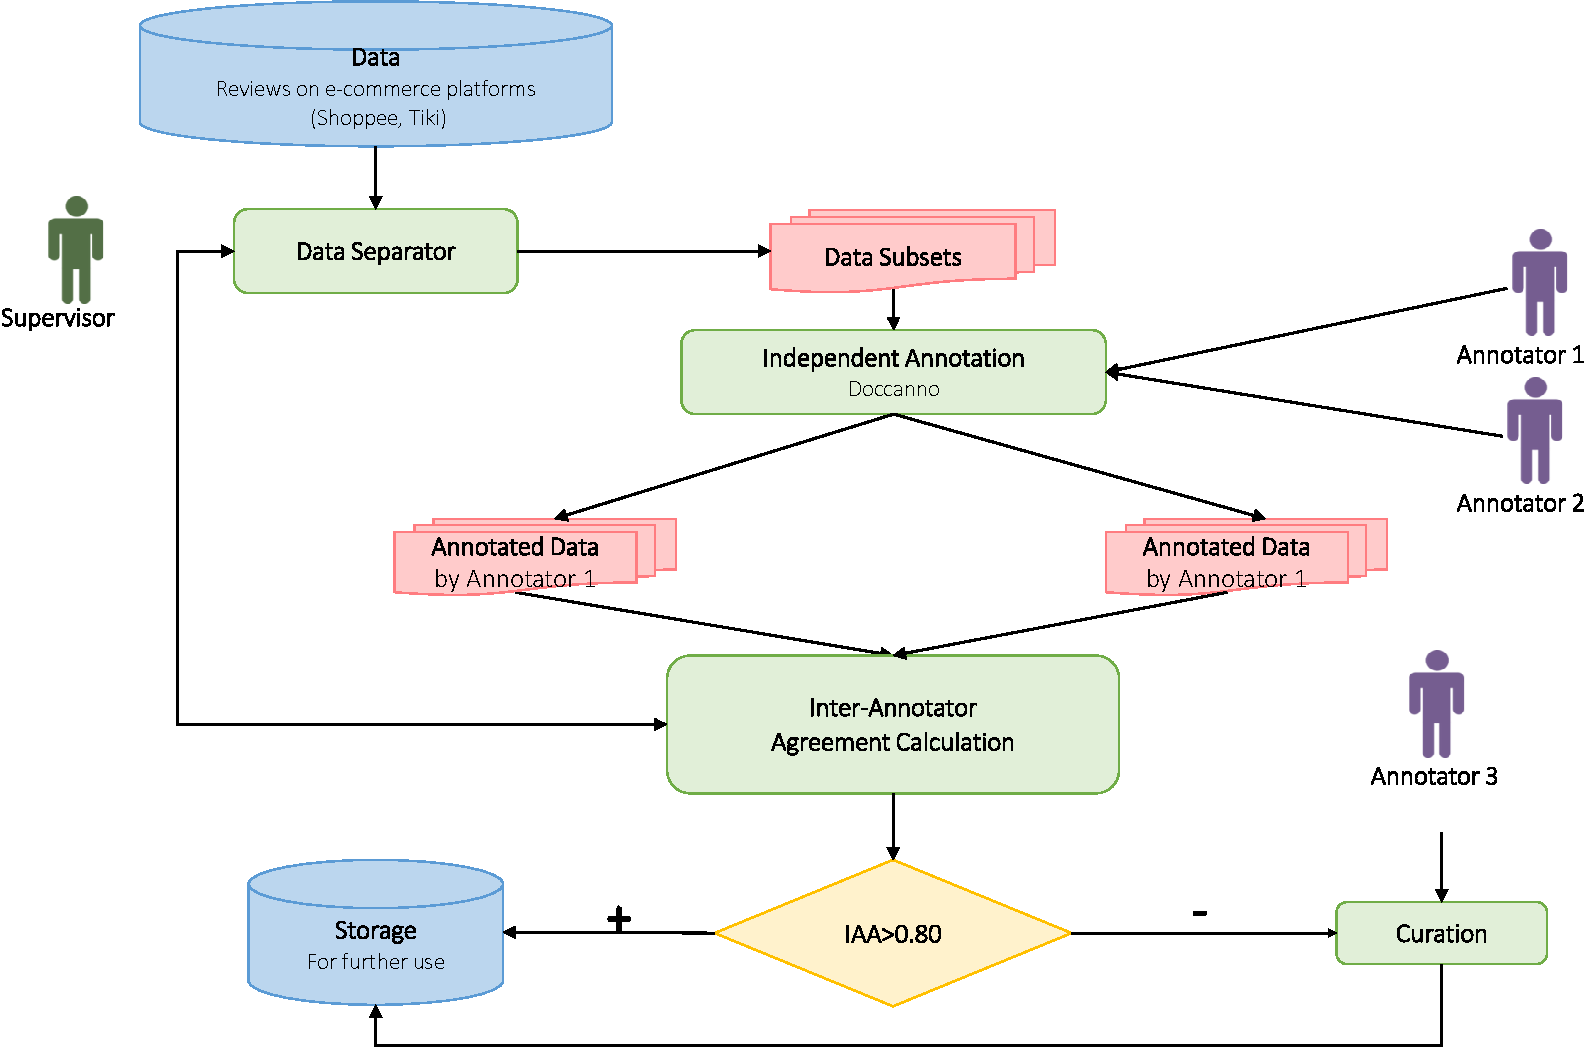
\includegraphics[width=\linewidth]{Chapter2/Figs/annotation.pdf}
	\caption{Data Annotation process}
	\label{fig:annotation}
\end{figure}

Data then separated in subsets, each of them was then evaluated and labeled by 2 annotators independently. Next, we measured the agreement between two annotators, if the result is too low (Inter-Annotator Agreement or IAA \(<\) 0.8), manually reviewing – process will be applied. The labeled data then stored as input for Pre-processing step. 

% -------------------------------------------------------------------
% Dataset Analysis
% -------------------------------------------------------------------
\section{Dataset Analysis}
\label{sec:data-analysis}
\paragraph{}
The statistics of Vietnamese E-commerce dataset (VECD) including Shopee and Tiki in two different domains:  Technology and Mother \& Baby are reported in figure 1 to 4. VECD consists of 3016 instances of Shopee Mother \& Baby, 2986 instances of Tiki , 3002 instances of Shopee Technology and 3236 instances of Tiki Technology, making up 12240 instances in total.

\begin{table}[h]
\centering
\begin{tabular}{|l|c|c|c|c|}
\hline
\multirow{2}{*}{}                                        & \multicolumn{2}{c|}{\textbf{Mother \& Baby}}           & \multicolumn{2}{c|}{\textbf{Technology}}                \\ \cline{2-5} 
                                                         & \textit{\textbf{Shopee}} & \textit{\textbf{Tiki}} & \textit{\textbf{Shopee}} & \textit{\textbf{Tiki}} \\ \hline
\multicolumn{1}{|c|}{\textbf{Total aspect}}              & 6                        & 6                      & 8                        & 8                      \\ \hline
\multicolumn{1}{|c|}{\textbf{Aspect count per sentence}} & 1.753234                 & 1.497347               & 2.087627                 & 1.746551               \\ \hline
\end{tabular}
\caption{The average number of aspects mentioned}
\end{table}

\begin{figure}[h]
	\centering
	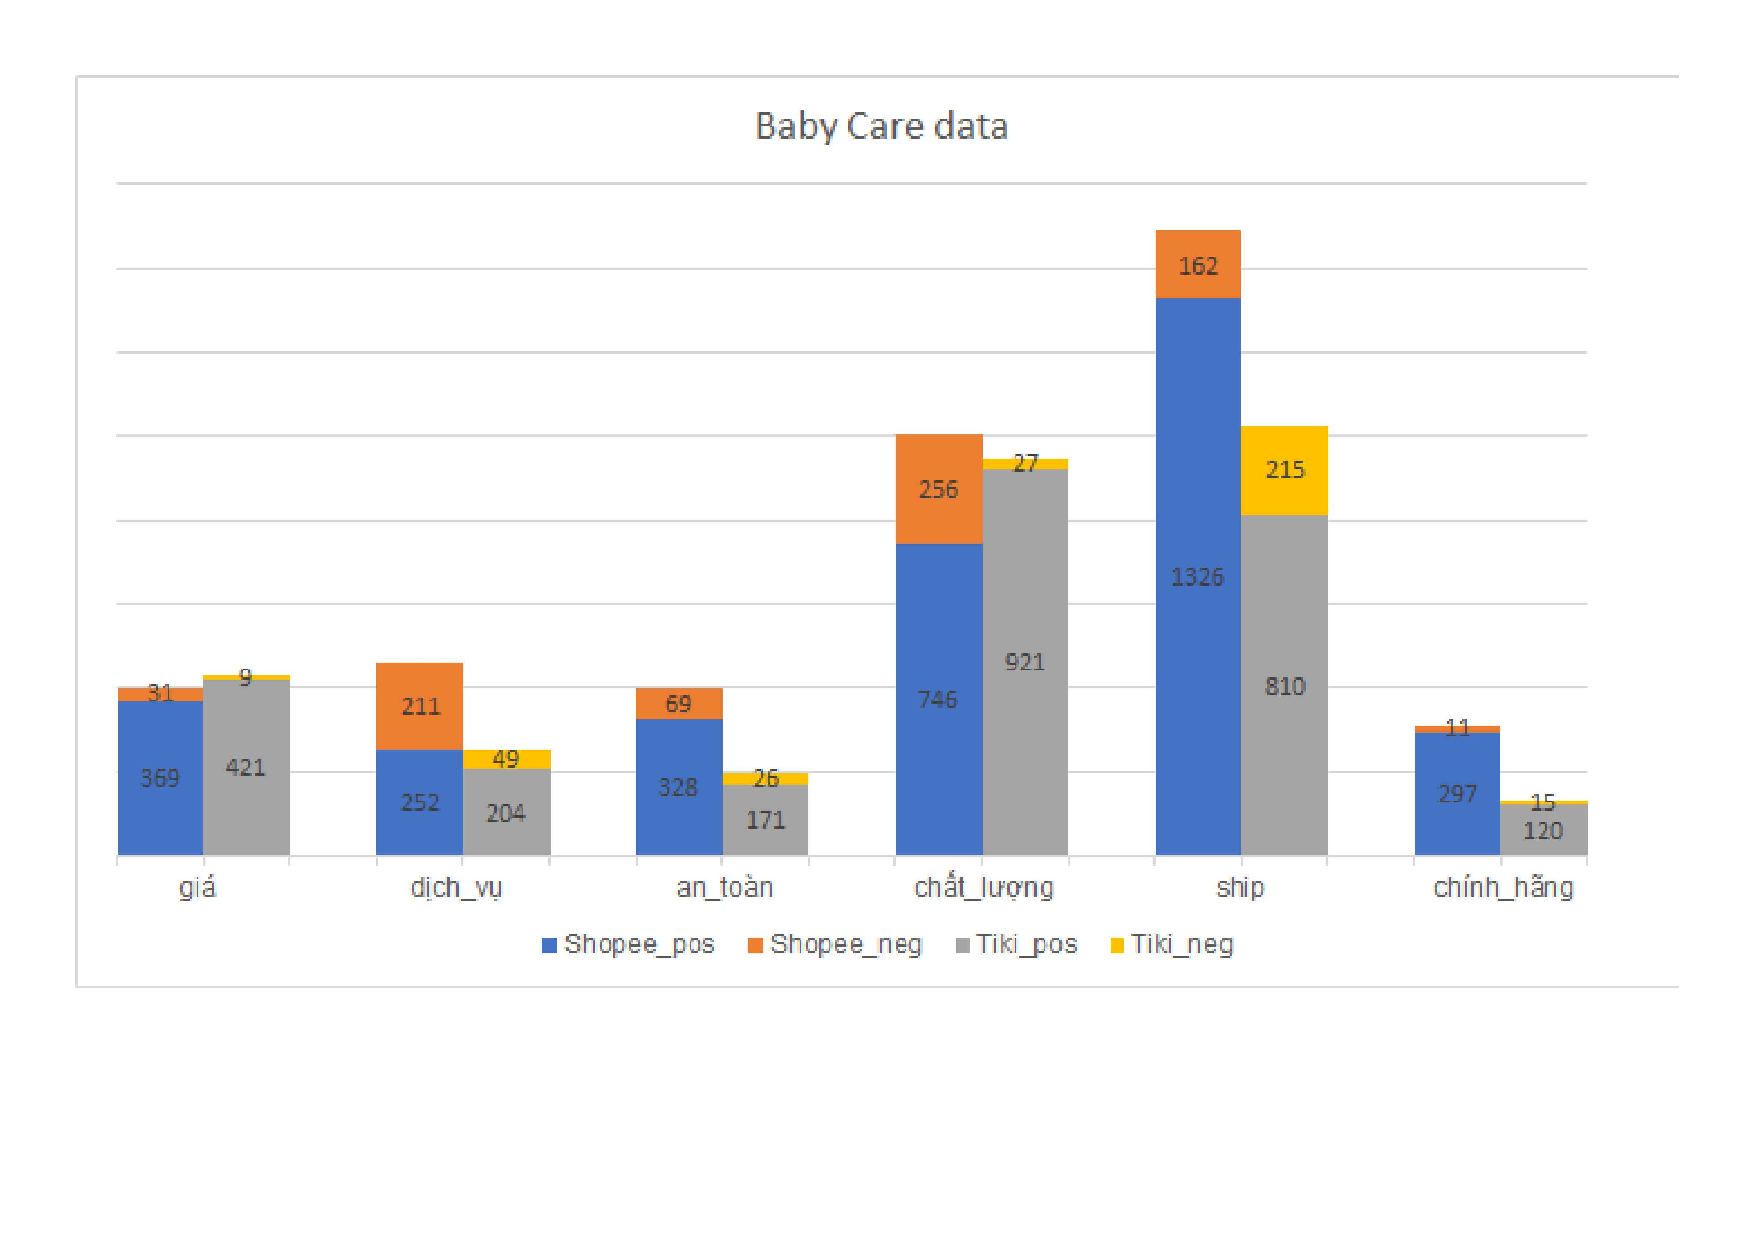
\includegraphics[width=\linewidth]{Chapter2/Figs/baby care.pdf}
	\caption{Mother \& Baby data statistics}
	\label{fig:baby}
\end{figure}

In Mother \& Baby domain, Shipping and Quality appear to be the most concerned aspects. Shopee has $1541$/$3216$ comments on Shipping and $773$/$3216$ comments on Quality, while in Tiki they are $972$/$2986$ and $1177$/$2986$ respectively. Authenticity only occasionally mentioned in Tiki's comments, just in $131$ cases while the others are mentioned in over $200$ comments, in both platforms, including Authenticity mentioned in Shopee.

Similarly, in Technology domain, Appearance is frequently mentioned in Shopee while it is Shipping in Tiki. More specifically $1064$ out of $3002$ comments on Shopee have information relating to products’ appearance, compared to $1021$ out of $3236$ comments on Tiki having information about Shipping. Price and Authenticity are the most imbalanced aspects, with only $4$ negative comments on Price and $12$ negative comments on Authenticity in Shopee while in Tiki the figures are $31$ and $24$, respectively. In Tiki, although the number of comments on Service, Hardware, Performance and Accessories is comparatively low, the data on these aspects are relatively balanced, with the difference below $16\%$.

\begin{figure}[]
	\centering
	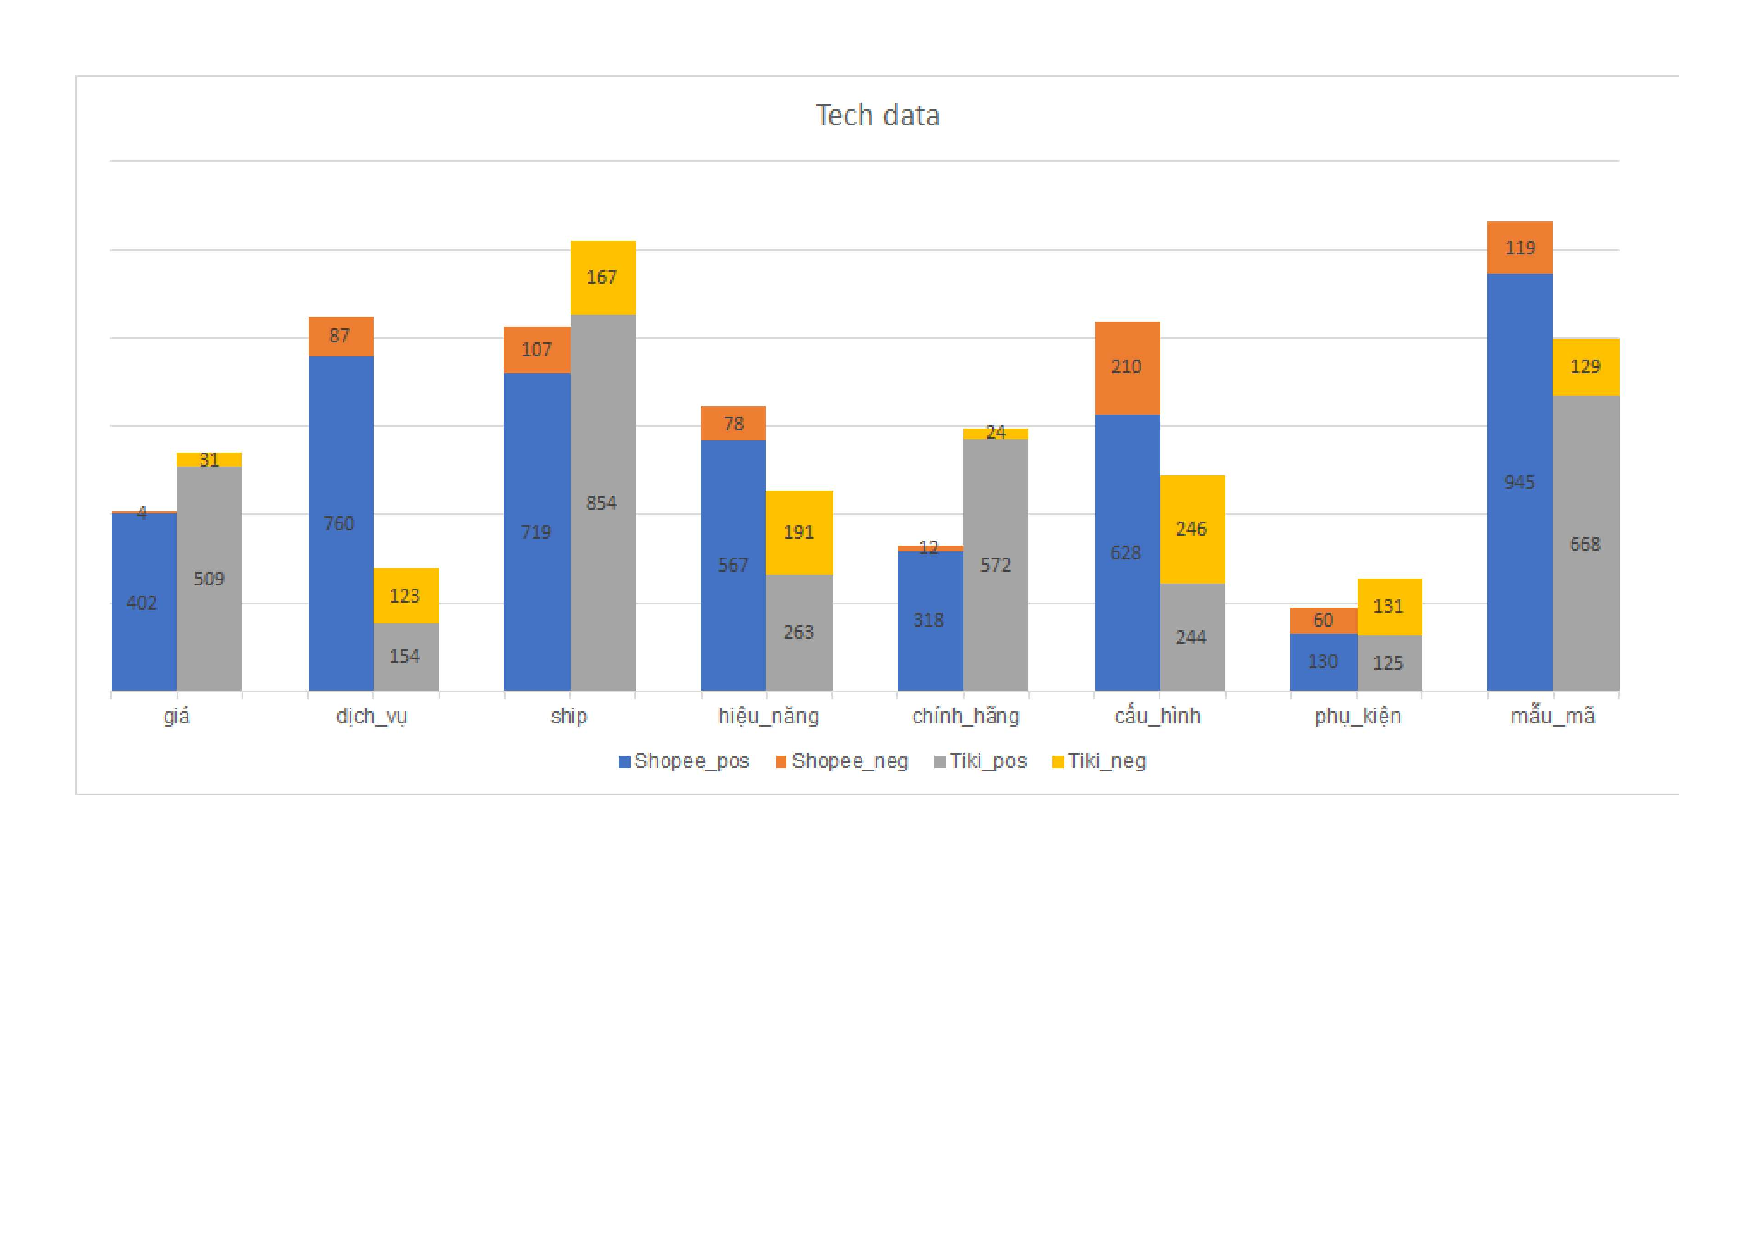
\includegraphics[width=\linewidth]{Chapter2/Figs/tech data.pdf}
	\caption{Technology data statistics}
	\label{fig:tech}
\end{figure}













\chapter{Phương Thức}
\label{chap:Phương Thức}

Trong chương này, chúng tôi sẽ trình bày phương thức chuẩn bị dữ liệu hội thoại, 

\section{Chuẩn Bị Dữ Liệu}

Chúng ta xác định một cuộc trò chuyện $C=\{ \left(u_{i}, y_{i}\right)\}_{i=1}^{L}$, trong đó $L$ là số lượng các câu nói trong cuộc trò chuyện, $u_{i}$ là câu nói thứ $i^{th}$ trong $C$ và $y_{i}$ là nhãn đúng của $u_{i}$. 
Ở đây, $y_{i} \in \left\{1,2,\cdots, c\right\}$ và $c$ là tổng số nhãn. 
Mỗi câu nói $u_{i}$ của người nói $p_{s(u_i)}$, trong đó hàm $s(\cdot)$ ánh xạ chỉ số của câu nói vào người nói tương ứng. 

Cho mỗi câu nói $u_{i}$, chúng ta trích xuất đặc trưng đa mô hình $x_{i}=\{{x}_{i}^m\}_{m\in\{a, l, v\}}$. 
Ở đây, $x_{i}^a \in \mathbb{R}^{d_a}$, $x_{i}^l \in \mathbb{R}^{d_l}$ and $x_{i}^v \in \mathbb{R}^{d_v}$ là các đặc trưng mức câu nói của các mô hình âm thanh, từ vựng và hình ảnh tương ứng.
Và $\{d_{m}\}_{m\in\{a, l, v\}}$ là chiều của đặc trưng của mỗi mô hình.

Để tạo ra các trường hợp mất mô hình giống như trong thế giới thực, chúng ta sẽ loại bỏ ngẫu nhiên một số mô hình, nhưng đảm bảo ít nhất có một mô hình cho mỗi mẫu, theo các công trình trước đó.

% \cite{chen2020hgmf, zhang2022deep}. - có cite

Do đó, một tập dữ liệu $M$ không hoàn thiện có $\left(2^{M}-1\right)$ mẫu thiếu sót khác nhau. 
Hình \ref{Figure2} minh họa một tập dữ liệu trimodal ($M=3$) với bảy mẫu thiếu sót. 
Giả sử $\sigma_{i}$ là mẫu thiếu sót của $u_{i}$ và $\phi(\cdot)$ là một hàm mô tả mỗi mẫu thiếu sót với các chế độ có sẵn. 
Biểu diễn không hoàn thiện của $u_{i}$ được đánh dấu là $\widetilde{x}_{i}=\{{\lambda}_{i}^m{x}_{i}^m\}_{m\in\{a, l, v\}}$, trong đó ${\lambda}_{i}^m$ được định nghĩa như sau:

\begin{equation}
	\label{eq1}
	{\lambda}_{i}^m=\begin{cases}
	1, m\in\phi(\sigma_{i}) \\
	0, m\notin\phi(\sigma_{i}) \\
	\end{cases}
\end{equation}




\section{Mã Hoá Thông Tin Ngữ Cảnh} 

Như đã đề cập ở trên, thông tin ngữ cảnh hội thoại là quan trọng để dự đoán nhãn cảm xúc của mỗi lời nói. Vì vậy, việc mã hóa thông tin ngữ cảnh vào biểu diễn tính năng của lời nói là có lợi. Chúng ta tạo ra mã hóa tính năng của lời nói được nhận thông tin ngữ cảnh cho mỗi modality qua mã hóa modality tương ứng. Cụ thể, chúng ta sử dụng mạng LSTM kết hợp hai chiều để mã hóa thông tin ngữ cảnh liên tục cho modality văn bản. Đối với modality âm thanh và hình ảnh, chúng ta sử dụng mạng kết nối đầy đủ. Mã hóa tính năng của lời nói được nhận thông tin ngữ cảnh có thể biểu diễn như sau:

\begin{small}
\begin{equation}
\begin{aligned}
    \centering
    &h_{i}^t = [\overrightarrow{\mathrm{LSTM}}(u_{i}^t,h_{i-1}^t),\overleftarrow{\mathrm{LSTM}}(u_{i}^t,h_{i+1}^t)] \\
    &h_{i}^a = W_{e}^a u_{i}^a+b_{i}^a \\
    &h_{i}^v = W_{e}^v u_{i}^v+b_{i}^v
\end{aligned}
\end{equation}
\end{small}
trong đó $u_{i}^a$, $u_{i}^v$ , $u_{i}^t$  là biểu diễn tính năng thô cảnh của câu thoại $i$ từ modality âm thanh, hình ảnh và văn bản, tương ứng. Mã hóa modality xuất ra mã hóa tính năng thô cảnh cho các modality $h_{i}^a$, $h_{i}^v$, and $h_{i}^t$ tương ứng.





\chapter{Experiments and Results}
\label{chap:experiments}

\section{Experiment Setup}
\subsection{Experimental Data}
In preparation to evaluate the effectiveness of our model, we proposed experiments on the Baby Care dataset collected from Shopee and Tiki, which has been described previously.
\subsection{Baseline Methods}
We compare various combinations of classifiers and different representation methods to figure out which one is most effective for our situation. The evaluation process is:

(1) Classic models: Logistics Regression, Random Forest, Decision Tree, Naive Bayes, K-nearest Neighbors and Support Vector Machine combine with different representation methods: One-Hot, Chi-Squared, PhoBERT.

(2) Logistics Regression with different representation methods.

(3) General comparison with/without WWL to find out the best model.

\subsection{Evaluation Metrics}
\paragraph{Precision}
Precision is the ratio of correctly predicted positive observations to the total predicted positive observations.
High precision relates to the low false positive rate.
\begin{equation}
Precision = \frac{TP}{TP+FP}
\end{equation}
where
\begin{description}
\item[] \(TP\) = True Positive - correctly predicted positive values which means that the value of actual class is 1 and value of predicted class is also 1.
\item[] \(FP\) = False Positive - actual class is 0 and predicted class is 1.
\end{description}
\paragraph{Recall}
Recall is the ratio of correctly predicted positive observations to the all observations in actual class.
High recall is synonymous with the low false negative rate.
\begin{equation}
Recall = \frac{TP}{TP+FN}
\end{equation}
where
\begin{description}
\item[] \(FP\) = False Negative - actual class is 1 and predicted class is 0.
\end{description}
\paragraph{F1-sscore}
The F1 is a way of combining the precision and recall of the model. The higher the F1 score the better, with 0 being the worst possible, which means the precision or recall is zero; and 1 being the best, indicating perfect precision and recall.
F1-score is defined as the harmonic mean of the model's precision and recall.
\begin{equation}
F1 = \frac{2*Precision*Recall}{Precision+Recall}
\end{equation}


\paragraph{Micro-average and Macro-average Performance}
Micro Average and Macro Average Performance are used to evaluate multi-label classification model. A macro-average will compute the metric independently for each class and then take the average, whereas a micro-average will aggregate the contributions of all classes to compute the average metric.
Micro- and macro-average for Precision, Recall and F1-score is calculated by the formulas as shown in the Equations from~\ref{eq:macro} to~\ref{eq:micro}.

\begin{align}
    P_{macro} = \frac{\sum_{i} P_{i}}{N}
    \,\,\,\,\,\,\,\,\,\,\,\,
    R_{macro} = \frac{\sum_{i} R_{i}}{N}
    \,\,\,\,\,\,\,\,\,\,\,\,
    F1_{macro} = \frac{\sum_{i} F1_{i}}{N}
    \label{eq:macro}
\end{align}

\begin{align}
    P_{micro} &= \frac{\sum_{j}^{} TP_{j}}{\sum_{j} TP_{j}+\sum_{j} FP_{j}} \\
    R_{micro} &= \frac{\sum_{j}^{} TP_{j}}{\sum_{j} TP_{j}+\sum_{j} FN_{j}} \\
    F1_{micro} &= \frac{2*P_{micro}*R_{micro}}{P_{micro}+R_{micro}}
    \label{eq:micro}
\end{align}

\section{Experiment Result and Analysis}
\label{sec:experiment-result}

In context of facing imbalance data (positive outnumbered negative) as analysed in Section~\ref{sec:data-analysis}, we appreciate the results of class negative in particular. 
In this section, we will use  Micro/Macro-average metrics calculated for negative class as the measure of evaluation.
\subsection{Classic Models with One-Hot Representation Method.}
With the OH data representation method, we use the Mother \& Baby data collected from Tiki as the input data for traditional machine learning models. Applying this simple method surprisingly brings fairly good results for such unbalanced data (compared to the methods below) but the negative value of some aspects is not yet assigned.

Based on the results of applying models, we find that the model using the LR method has the most outstanding results. We will use a combination of this method and the data representation methods below to compare results.

% \begin{table}[h]
% \centering
% \begin{tabular}{|c|c|c|c|c|c|c|c|c|}
% \hline
%             & \textit{\textbf{price}} & \textit{\textbf{service}} & \textit{\textbf{safety}} & \textit{\textbf{quality}} & \textit{\textbf{delivery}} & \textit{\textbf{authenticity}} & \textit{\textbf{micro}} & \textit{\textbf{macro}} \\ \hline
% \textbf{P}  & 1,000                   & 0,653                     & 0,875                    & 0,698                     & 0,767                      & \textbf{0,000}                 & 0,701                   & 0,665                   \\ \hline
% \textbf{R}  & 0,200                   & 0,744                     & 0,538                    & 0,545                     & 0,311                      & \textbf{0,000}                 & 0,475                   & 0,390                   \\ \hline
% \textbf{F1} & 0,333                   & 0,696                     & 0,667                    & 0,612                     & 0,442                      & \textbf{0,000}                 & 0,566                   & 0,458                   \\ \hline
% \end{tabular}
% \caption{OH + LR statistics}
% \end{table}

Evaluation results are illustrated in table~\ref{tab:ohneg}.

% \begin{table}[h]
% \centering
% \begin{tabular}{|c|c|c|c|c|c|c|}
% \hline
% \multicolumn{1}{|l|}{} & \textit{\textbf{SVM}} & \textit{\textbf{DT}} & \textit{\textbf{KN}} & \textit{\textbf{LR}} & \textit{\textbf{NB}} & \textit{\textbf{RF}} \\ \hline
% \textbf{micro-p}  & 0,865 & 0,904 & 0,884 & 0,936          & 0,879 & 0,955 \\ \hline
% \textbf{micro-r}  & 0,974 & 0,876 & 0,989 & 0,973          & 0,993 & 0,657 \\ \hline
% \textbf{micro-f1} & 0,916 & 0,890 & 0,934 & \textbf{0,954} & 0,932 & 0,778 \\ \hline
% \textbf{macro-p}  & 0,869 & 0,909 & 0,895 & 0,937          & 0,894 & 0,960 \\ \hline
% \textbf{macro-r}  & 0,949 & 0,874 & 0,987 & 0,972          & 0,987 & 0,686 \\ \hline
% \textbf{macro-f1} & 0,906 & 0,890 & 0,939 & \textbf{0,954} & 0,938 & 0,797 \\ \hline
% \end{tabular}
% \caption{Micro/Macro Average for class positive of OH + traditional models}
% \label{tab:ohpos}
% \end{table}

\begin{table}[h]
\centering
\begin{tabular}{|c|c|c|c|c|c|c|}
\hline
\multicolumn{1}{|l|}{} &
  \multicolumn{1}{c|}{\textit{\textbf{SVM}}} &
  \multicolumn{1}{c|}{\textit{\textbf{DT}}} &
  \multicolumn{1}{c|}{\textit{\textbf{KN}}} &
  \multicolumn{1}{c|}{\textit{\textbf{LR}}} &
  \multicolumn{1}{c|}{\textit{\textbf{NB}}} &
  \multicolumn{1}{c|}{\textit{\textbf{RF}}} \\ \hline
\textbf{micro-p}  & 0,587 &0,622 &0,541 &0,810 &0,205 &0,818 \\ \hline
\textbf{micro-r}  & 0,228 &0,599 &0,370 &0,525 &0,746 &0,500 \\ \hline
\textbf{micro-f1} & 0,329 &0,610 &0,440 &\textbf{0,637} &0,322 &0,621 \\ \hline
\textbf{macro-p}  & 0,330 &0,422 &0,389 &0,541 &0,183 &0,548 \\ \hline
\textbf{macro-r}  & 0,159 &0,397 &0,258 &0,351 &0,641 &0,329 \\ \hline
\textbf{macro-f1} & 0,176 &0,406 &0,299 &0,405 &0,277 &0,395 \\ \hline
\end{tabular}
\caption{Micro/Macro-average for class negative of OH + traditional models}
\label{tab:ohneg}
\end{table}


% \paragraph{Chi-Squared}

% This method works well with DT, RF, LR. But the negative class of some aspects is still not assigned. For example, as the model using LR, the results are shown as table below.

% Other models also suffer from defects, but the results have been improved.

% \begin{table}[h]
% \centering
% \begin{tabular}{|c|c|c|c|c|c|c|c|c|}
% \hline
% \multicolumn{1}{|l|}{} & \textit{\textbf{price}} & \textit{\textbf{service}} & \textit{\textbf{safety}} & \textit{\textbf{quality}} & \textit{\textbf{delivery}} & \textit{\textbf{authenticity}} & \textit{\textbf{micro}} & \textit{\textbf{macro}} \\ \hline
% \textbf{P}             & 0,500          & 0,723                     & 0,500                    & 0,537                     & 0,663                  & \textbf{0,250}                 & 0,616                   & 0,529                   \\ \hline
% \textbf{R}             & 0,600          & 0,791                     & 0,538                    & 0,527                     & 0,716                  & \textbf{0,333}                 & 0,657                   & 0,584                   \\ \hline
% \textbf{F1}            & 0,545          & 0,756                     & 0,519                    & 0,532                     & 0,688                  & \textbf{0,286}                 & 0,636                   & 0,554                   \\ \hline
% \end{tabular}
% \caption{CS + DT statistics}
% \end{table}
% Micro- and macro-average Performance of Precision, Recall and F1-score is illustrated in table~\ref{tab:chipos} and table~\ref{tab:chineg}. 

% \begin{table}[h]
% \centering
% \begin{tabular}{|c|c|c|c|c|c|c|}
% \hline
% \multicolumn{1}{|l|}{} & \textit{\textbf{SVM}} & \textit{\textbf{DT}} & \textit{\textbf{KN}} & \textit{\textbf{LR}} & \textit{\textbf{NB}} & \textit{\textbf{RF}} \\ \hline
% \textbf{micro-p}       & 0,865                 & 0,935                & 0,905                & 0,919                & \textbf{0,942}       & 0,921                \\ \hline
% \textbf{micro-p}       & 0,906                                      & 0,935                                     & 0,905                                     & 0,919                                     & \textbf{0,942}                            & 0,921                                     \\ \hline
% \textbf{micro-r}       & \textbf{0,991}                             & 0,930                                     & 0,946                                     & 0,964                                     & 0,595                                     & 0,964                                     \\ \hline
% \textbf{micro-f1}      & \textbf{0,946}                             & 0,932                                     & 0,925                                     & 0,941                                     & 0,729                                     & 0,942                                     \\ \hline
% \textbf{macro-p}       & 0,912                                      & 0,942                                     & 0,908                                     & 0,930                                     & \textbf{0,950}                            & 0,925                                     \\ \hline
% \textbf{macro-r}       & \textbf{0,988}                             & 0,927                                     & 0,934                                     & 0,958                                     & 0,664                                     & 0,962                                     \\ \hline
% \textbf{macro-f1}      & \textbf{0,948}                             & 0,934                                     & 0,921                                     & 0,944                                     & 0,772                                     & 0,943                                     \\ \hline
% \end{tabular}
% \caption{Micro/Macro Average for class positive of CS + traditional models}
% \label{tab:chipos}
% \end{table}

% \begin{table}[h]
% \centering
% \begin{tabular}{|c|c|c|c|c|c|c|}
% \hline
%                   & \textit{\textbf{SVM}} & \textit{\textbf{DT}} & \textit{\textbf{KN}} & \textit{\textbf{LR}} & \textit{\textbf{RF}} & \textit{\textbf{NB}} \\ \hline
% \textbf{micro-p}       & 0,865                                      & 0,904                                     & 0,884                                     & 0,936                                     & 0,879                                     & \textbf{0,955}                            \\ \hline
% \textbf{micro-r}       & 0,974                                      & 0,876                                     & 0,989                                     & 0,973                                     & \textbf{0,993}                            & 0,657                                     \\ \hline
% \textbf{micro-f1}      & 0,916                                      & 0,890                                     & 0,934                                     & \textbf{0,954}                            & 0,932                                     & 0,778                                     \\ \hline
% \textbf{macro-p}       & 0,869                                      & 0,909                                     & 0,895                                     & 0,937                                     & 0,894                                     & \textbf{0,960}                            \\ \hline
% \textbf{macro-r}       & 0,949                                      & 0,874                                     & 0,987                                     & 0,972                                     & \textbf{0,987}                            & 0,686                                     \\ \hline
% \textbf{macro-f1}      & 0,906                                      & 0,890                                     & 0,939                                     & \textbf{0,954}                            & 0,938                                     & 0,797                                     \\ \hline
% \end{tabular}
% \caption{Micro/Macro Average for class negative of CS + traditional models}
% \label{tab:chineg}
% \end{table}

% % \paragraph{PhoBERT} With the data representation using PhoBERT, we compare with DL methods: CNN and MLP. The results are very noticeable but still lower than the DL model.

% % Micro- and macro-average Performance of Precision, Recall and F1-score is illustrated below. 

% % \begin{table}[h]
% % \centering
% % \begin{tabular}{|c|c|c|c|c|c|c|c|c|}
% % \hline
% %  & \textit{\textbf{SVM}} & \textit{\textbf{DT}} & \textit{\textbf{KN}} & \textit{\textbf{LR}} & \textit{\textbf{RF}} & \textit{\textbf{CNN}} & \textit{\textbf{MLP}} \\ \hline
% % \textbf{micro-p}  & 0,940                 & 0,935                & 0,919                & 0,943                & 0,939                & \textbf{0,945}        & 0,930                 \\ \hline
% % \textbf{micro-r}  & 0,941                 & 0,930                & 0,962                & 0,957                & 0,981                & \textbf{0,981}        & 0,974                 \\ \hline
% % \textbf{micro-f1} & 0,940                 & 0,932                & 0,940                & 0,950                & 0,959                & \textbf{0,963}        & 0,951                 \\ \hline
% % \textbf{macro-p}  & 0,944                 & 0,942                & 0,926                & \textbf{0,947}       & 0,940                & 0,925                 & 0,925                 \\ \hline
% % \textbf{macro-r}  & 0,939                 & 0,927                & 0,961                & 0,950                & 0,977                & \textbf{0,986}        & 0,952                 \\ \hline
% % \textbf{macro-f1} & 0,942                 & 0,934                & 0,943                & 0,948                & \textbf{0,958}       & 0,954                 & 0,946                 \\ \hline
% % \end{tabular}
% % \caption{Micro/Macro Average for class positive of PhoBERT + traditional models and DL models}
% % \label{tab:phopos}
% % \end{table}

% % \begin{table}[h]
% % \centering
% % \begin{tabular}{|c|c|c|c|c|c|c|c|}
% % \hline
% %  & \textit{\textbf{SVM}} & \textit{\textbf{DT}} & \textit{\textbf{KN}} & \textit{\textbf{LR}} & \textit{\textbf{RF}} & \textit{\textbf{CNN}} & \textit{\textbf{MLP}} \\ \hline
% % \textbf{micro-p}  & \textbf{0,863}        & 0,573                & 0,552                & 0,778                & 0,703                & 0,818                 & 0,454                 \\ \hline
% % \textbf{micro-r}  & 0,359                 & 0,631                & 0,404                & 0,583                & 0,490                & 0,643                 & \textbf{0,767}        \\ \hline
% % \textbf{micro-f1} & 0,507                 & 0,601                & 0,466                & 0,667                & 0,577                & \textbf{0,714}        & 0,571                 \\ \hline
% % \textbf{macro-p}  & 0,595                 & 0,552                & 0,396                & 0,522                & 0,702                & \textbf{0,734}        & 0,458                 \\ \hline
% % \textbf{macro-r}  & 0,251                 & \textbf{0,686}       & 0,309                & 0,418                & 0,437                & 0,430                 & 0,671                 \\ \hline
% % \textbf{macro-f1} & 0,331                 & \textbf{0,607}       & 0,338                & 0,462                & 0,514                & 0,475                 & 0,551                 \\ \hline
% % \end{tabular}
% % \caption{Micro/Macro Average for class negative of PhoBERT + traditional models and DL models}
% % \label{tab:phoneg}
% % \end{table}

% \paragraph{Word-Window Locating + Chi-Squared}
% The model that uses WWL before data representation gives desirable results. There is still the problem of the negative class with some unassigned aspects, but this has been greatly improved in comparison to traditional models.

% \begin{table}[]
% \centering
% \begin{tabular}{|c|c|c|c|c|c|c|}
% \hline
%  & \textit{\textbf{SVM}} & \textit{\textbf{DT}} & \textit{\textbf{KN}} & \textit{\textbf{LR}} & \textit{\textbf{NB}} & \textit{\textbf{NB}} \\ \hline
% \textbf{micro-p}  & 0,930          & 0,933 & 0,913 & \textbf{0,945} & 0,938 & 0,920 \\ \hline
% \textbf{micro-r}  & \textbf{0,986} & 0,940 & 0,975 & 0,973          & 0,948 & 0,983 \\ \hline
% \textbf{micro-f1} & 0,957          & 0,936 & 0,943 & \textbf{0,959} & 0,943 & 0,951 \\ \hline
% \textbf{macro-p}  & 0,921          & 0,922 & 0,907 & \textbf{0,936} & 0,929 & 0,916 \\ \hline
% \textbf{macro-r}  & \textbf{0,982} & 0,935 & 0,977 & 0,971          & 0,960 & 0,980 \\ \hline
% \textbf{macro-f1} & 0,950          & 0,928 & 0,940 & \textbf{0,953} & 0,943 & 0,947 \\ \hline
% \end{tabular}
% \caption{Micro/Macro Average for class positive of WWL + CS}
% \end{table}

% \begin{table}[]
% \centering
% \begin{tabular}{|c|c|c|c|c|c|c|}
% \hline
%  & \textit{\textbf{SVM}} & \textit{\textbf{DT}} & \textit{\textbf{KN}} & \textit{\textbf{LR}} & \textit{\textbf{NB}} & \textit{\textbf{NB}} \\ \hline
% \textbf{micro-p}  & 0,850 & 0,622 & 0,759 & 0,835          & 0,705 & \textbf{0,861} \\ \hline
% \textbf{micro-r}  & 0,631 & 0,682 & 0,525 & \textbf{0,742} & 0,687 & 0,596          \\ \hline
% \textbf{micro-f1} & 0,725 & 0,651 & 0,621 & \textbf{0,786} & 0,696 & 0,704          \\ \hline
% \textbf{macro-p}  & 0,568 & 0,510 & 0,714 & \textbf{0,885} & 0,499 & 0,564          \\ \hline
% \textbf{macro-r}  & 0,428 & 0,573 & 0,355 & \textbf{0,578} & 0,458 & 0,392          \\ \hline
% \textbf{macro-f1} & 0,481 & 0,534 & 0,410 & \textbf{0,640} & 0,460 & 0,452          \\ \hline
% \end{tabular}
% \caption{Micro/Macro Average for class negative of WWL + CS}
% \end{table}

\subsection{Logistics Regression with Different Representation Methods}
We use the model using the LR method for comparison since it is the model with the best results as calculated above. Mother \& Baby data collected from Tiki are used to evaluated results among three different representation methods: PhoBERT, CS and OH.
OH and PhoBERT showed relatively good results, but in general CS has the best performance. Table~\ref{tab:lr} illustrates micro- and macro-average performance for class negative of LR with multiple representation methods.

\begin{table}[h]
\centering
\begin{tabular}{|c|c|c|c|c|c|c|}
\hline
                  & \textit{\textbf{PhoBERT}} & \textit{\textbf{CS}} & \textit{\textbf{OH}}\\ \hline
\textbf{micro-p}  & 0,764 & 0,704          & 0,810 \\ \hline
\textbf{micro-r}  & 0,540 & 0,660          & 0,525 \\ \hline
\textbf{micro-f1} & 0,633 & \textbf{0,682} & 0,637 \\ \hline
\textbf{macro-p}  & 0,506 & 0,560          & 0,541 \\ \hline
\textbf{macro-r}  & 0,368 & 0,532          & 0,351 \\ \hline
\textbf{macro-f1} & 0,423 & \textbf{0,545} & 0,405 \\ \hline
\end{tabular}
\caption{Micro/Macro-average for class negative of LR with representation methods}
\label{tab:lr}
\end{table}

\subsection{Chi-Squared with/without Word-Window Locating compared with CNN + PhoBERT}

\begin{table}[h]
\centering
\begin{tabular}{|c|c|c|c|c|}
\hline               
& \textit{\textbf{CS + WWL}} & \textit{\textbf{CS}} & \textit{\textbf{CNN + PhoBERT}}\\ \hline
\textbf{micro-p}  & 0,738          & 0,704 & 0,801          \\ \hline
\textbf{micro-r}  & 0,728          & 0,660 & 0,747          \\ \hline
\textbf{micro-f1} & 0,733          & 0,682 & \textbf{0,773} \\ \hline
\textbf{macro-p}  & 0,781          & 0,560 & 0,512          \\ \hline
\textbf{macro-r}  & 0,632          & 0,532 & 0,518          \\ \hline
\textbf{macro-f1} & \textbf{0,674} & 0,545 & 0,515          \\ \hline
\end{tabular}
\caption{Micro/Macro-average of CS with/without WWL and CNN + PhoBERT}
\label{tab:cswwl}
\end{table}

We continue to use the model using LR method to compare between CS, CS + WWL and CNN + PhoBERT. 

The results indicate that CS + WWL outperformed CS alone in every figures. In comparison of CS + WWL and CNN + PhoBERT, it is indicated that micro-F1 of CNN + PhoBERT is slightly better with a percentage of 4\% but CS + WWL surpassed CNN + PhoBERT with a significant percentage of 16\%.

Evaluation proves effective use of the WWL method.

Table~\ref{tab:cswwl} shows micro- and macro-average performance of CS with/without WWL and CNN + PhoBERT, while table~\ref{tab:allaspects} shows CS + WWL vs. CNN + PhoBERT detailed statistical results in all aspects.

\begin{table}[h]
\centering
\begin{tabular}{|c|c|c|c|c|c|c|c|}
\hline
\textbf{Method} & \textbf{Class} & \textbf{Price} & \textbf{Service} & \textbf{Safety} & \textbf{Quality} & \textbf{Delivery} & \textbf{Authenticity} \\ \hline
\multirow{2}{*}{\textbf{CS + WWL}} & Positive & 0.983          & 0.757 & 0.892 & 0.907 & 0.928 & 0.960          \\ \cline{2-8} 
                                   & Negative & 0.571          & 0.804 & 0.774 & 0.718 & 0.676 & 0.500          \\ \hline
\multirow{2}{*}{\textbf{CNN}}      & Positive & 0.978          & 0.875 & 0.759 & 0.940 & 0.943 & 0.943          \\ \cline{2-8} 
                                   & Negative & \textbf{0.000} & 0.884 & 0.632 & 0.792 & 0.763 & \textbf{0.000} \\ \hline
\end{tabular}
\caption{WWL + CS vs. CNN + PhoBERT detailed statistics in all aspects}
\label{tab:allaspects}
\end{table}

\subsection{WWL + CS detailed statistics in all domains}
Given the proportional difference between the positive and negative classes of different datasets in the domain and the data source in the item (item name), we find that the model uses WWL with the CS method of representing the level data showed quite stable results.
% We make comparisons between our approach and SVM-based approach proposed by (Thin et al., \cite{van2018transformation}), which results specified that our method performed better.
The statistical results are described in table~\ref{tab:detailneg}.

\begin{table}[h]
\centering
\begin{tabular}{|c|c|c|c|c|}
\hline
 & \textit{\textbf{mb\_tiki}} & \textit{\textbf{mb\_shopee}} & \textit{\textbf{tech\_tiki}} & \textit{\textbf{tech\_shopee}} \\ \hline
\textbf{micro-p}  & 0,738 & 0,615 & 0,707 & 0,709 \\ \hline
\textbf{micro-r}  & 0,728 & 0,635 & 0,621 & 0,629 \\ \hline
\textbf{micro-f1} & 0,733 & 0,625 & 0,661 & 0,667 \\ \hline
\textbf{macro-p}  & 0,781 & 0,541 & 0,582 & 0,593 \\ \hline
\textbf{macro-r}  & 0,632 & 0,462 & 0,510 & 0,572 \\ \hline
\textbf{macro-f1} & 0,674 & 0,482 & 0,540 & 0,545 \\ \hline
\end{tabular}
\caption{CS + WWL detailed statistics for class negative in all domains}
\label{tab:detailneg}
\end{table}

\subsection{Error Analysis}
\begin{itemize}
    \item Unbalanced data results affect model training leading to low results for the indicated aspect.
    \item Lack of summarized data.
    \item Errors occur in the data annotation phase due to manual process.
    \item The investigation of the data is not in-depth, yield threshold selected for locating not matching the data.
\end{itemize}

\section{Demonstrations}
\subsection{Data Visualization}
We use Kibana and Elasticsearch to analyze and visualize data based on their labels and polarity. Figure~\ref{fig:label} and~\ref{fig:keyword} shows how our dataset are visualized based on labels and keywords.

\begin{figure}[h]
	\centering
	
\includegraphics[width=\linewidth]{Chapter4/Figs/kibana1.png}
	\caption{Dataset visualization based on labels and polarity}
	\label{fig:label}
\end{figure}

\begin{figure}[h]
	\centering
	
\includegraphics[width=\linewidth]{Chapter4/Figs/kibana2.png}
	\caption{Dataset visualization based on keywords}
	\label{fig:keyword}
\end{figure}

\subsection{Web Application Demonstration}
With a view to bring the model into practical situation, we built a web interface for users to manipulate easily.
The users will put in data in two ways: insert each comment by the 'Add' button (figure~\ref{fig:tool1}) or import a CSV file containing comment data along with the respective aspect (figure~\ref{fig:tool2}).

\begin{figure}[h]
	\centering
	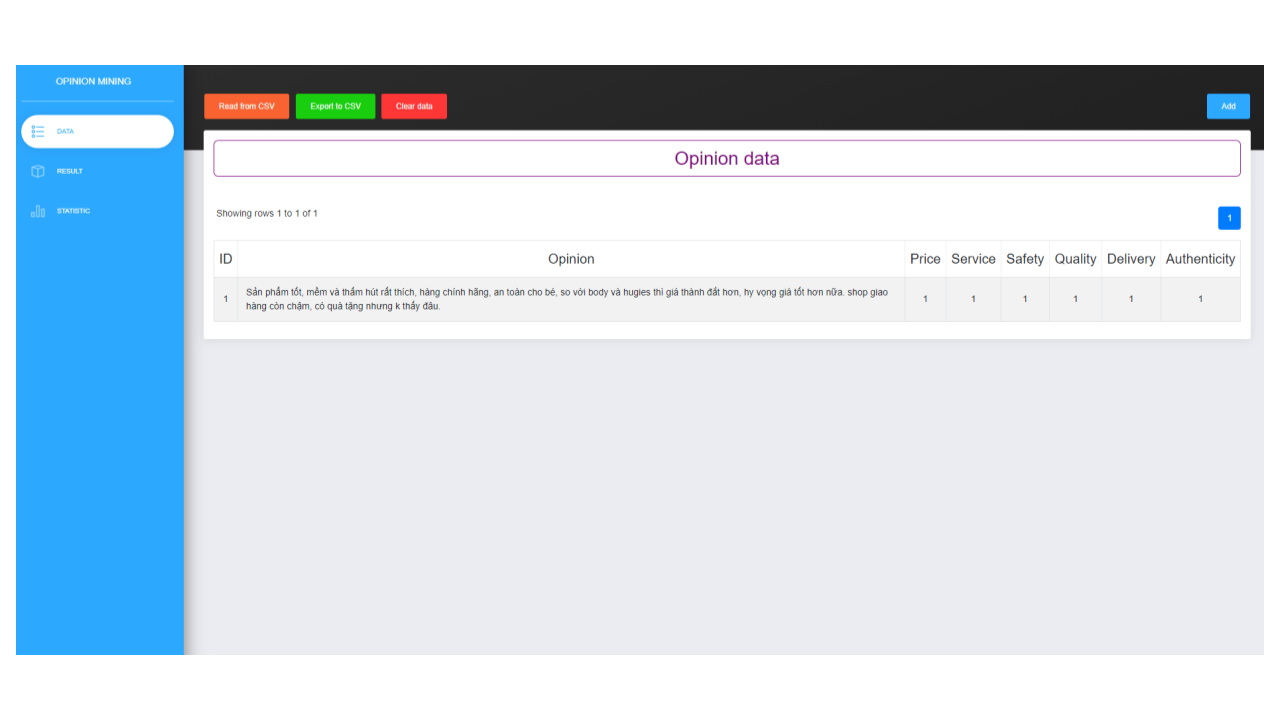
\includegraphics[width=\linewidth]{Chapter4/Figs/tool1.png}
	\caption{Insert comment by the 'Add' button}
	\label{fig:tool1}
\end{figure}

\begin{figure}[h]
	\centering
	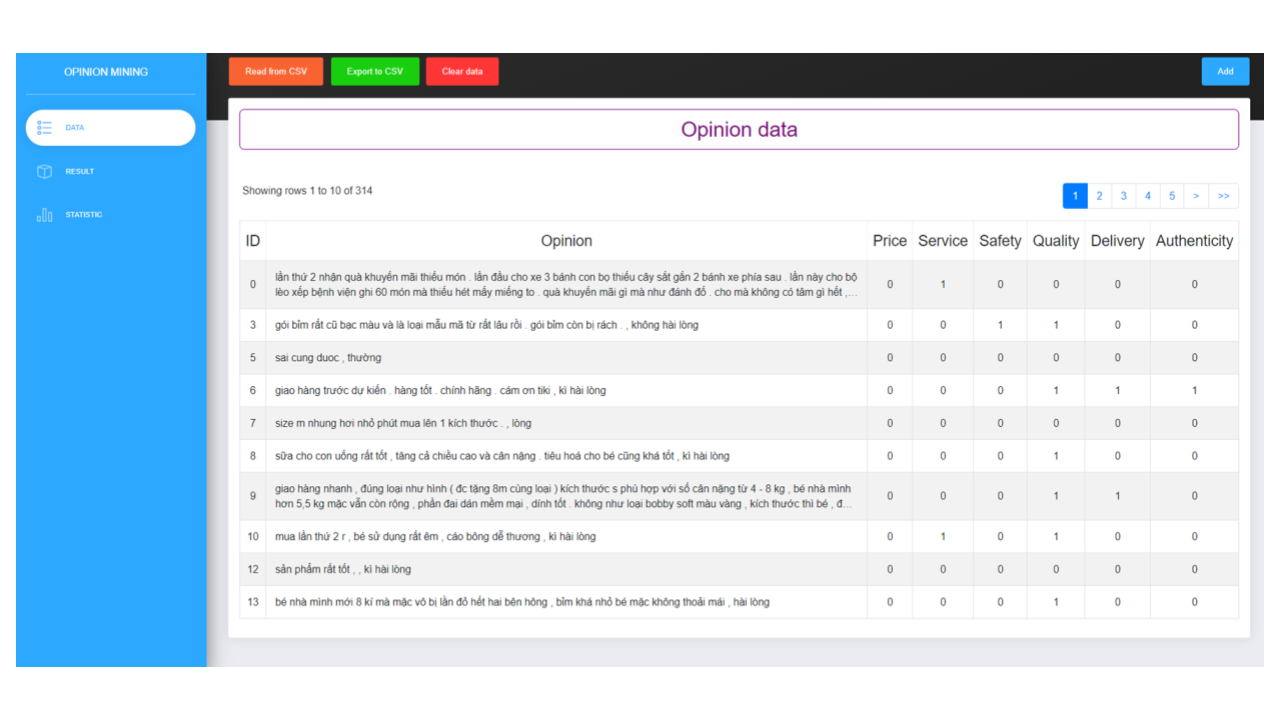
\includegraphics[width=\linewidth]{Chapter4/Figs/tool2.png}
	\caption{Insert comments by importing CSV file}
	\label{fig:tool2}
\end{figure}

The model runs when the user selects 'Result' button. The results as illustrated in figure~\ref{fig:tool3} and~\ref{fig:tool4} show -1 and 1 on the aspects that appear in the comment corresponding to the negative and positive emotions related to that aspect.

\begin{figure}[h]
	\centering
	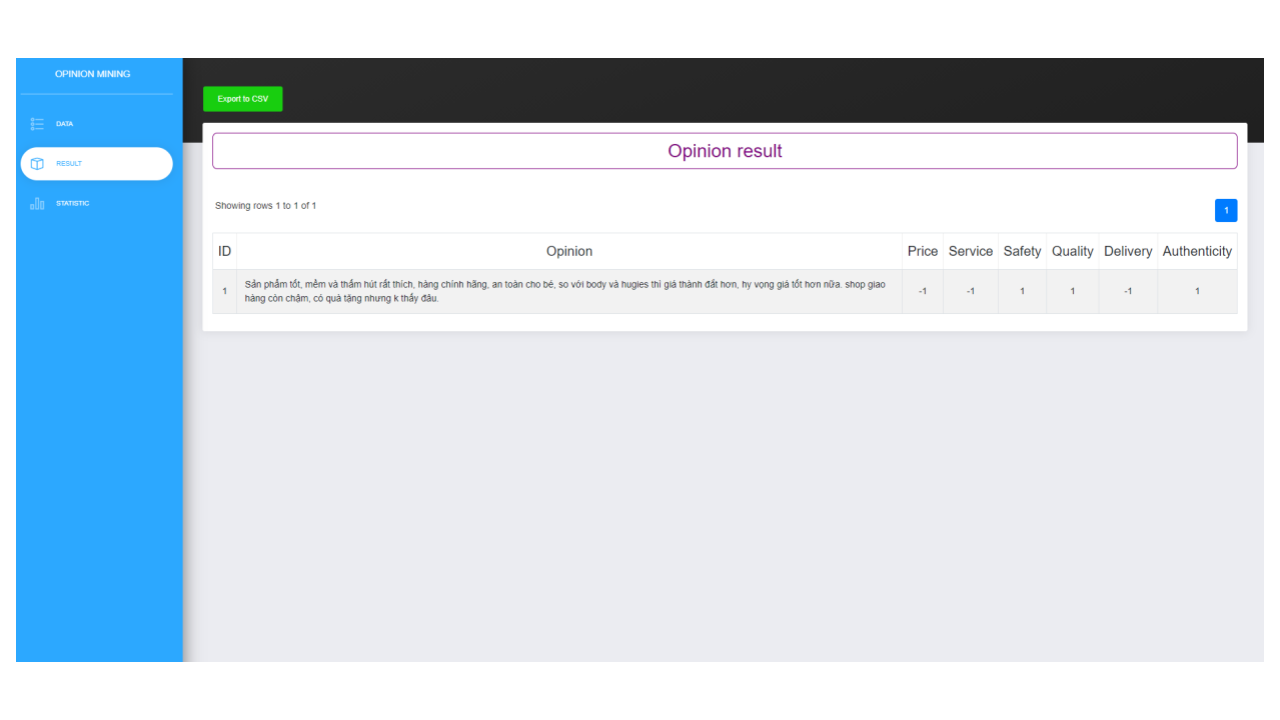
\includegraphics[width=\linewidth]{Chapter4/Figs/tool3.png}
	\caption{Model output when using 'Add" function}
	\label{fig:tool3}
\end{figure}

\begin{figure}[h]
	\centering
	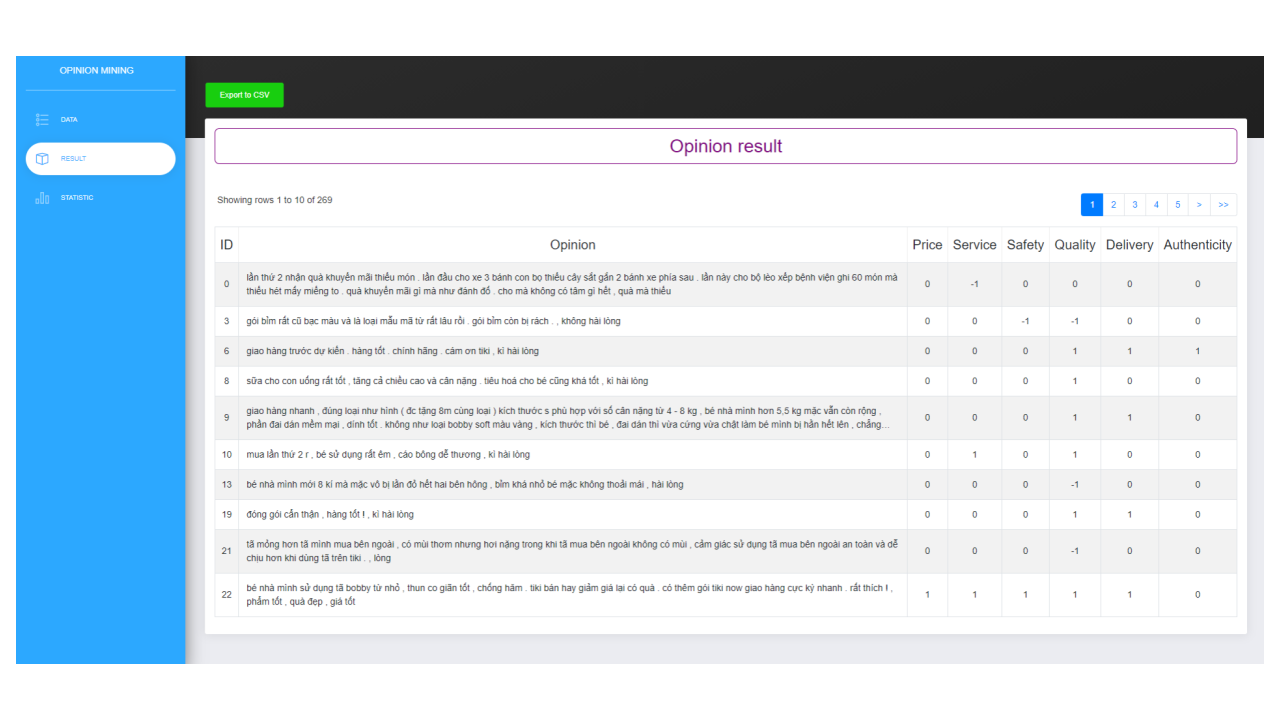
\includegraphics[width=\linewidth]{Chapter4/Figs/tool4.png}
	\caption{Model output when using 'Import" function}
	\label{fig:tool4}
\end{figure}

In addition, we have built a few functions for the web application such as showing detailed statistical results of positive and negative sentiment on each aspects, exporting results in CSV, PNG, etc. formats for data statistics and visualization.

\begin{figure}[h]
	\centering
	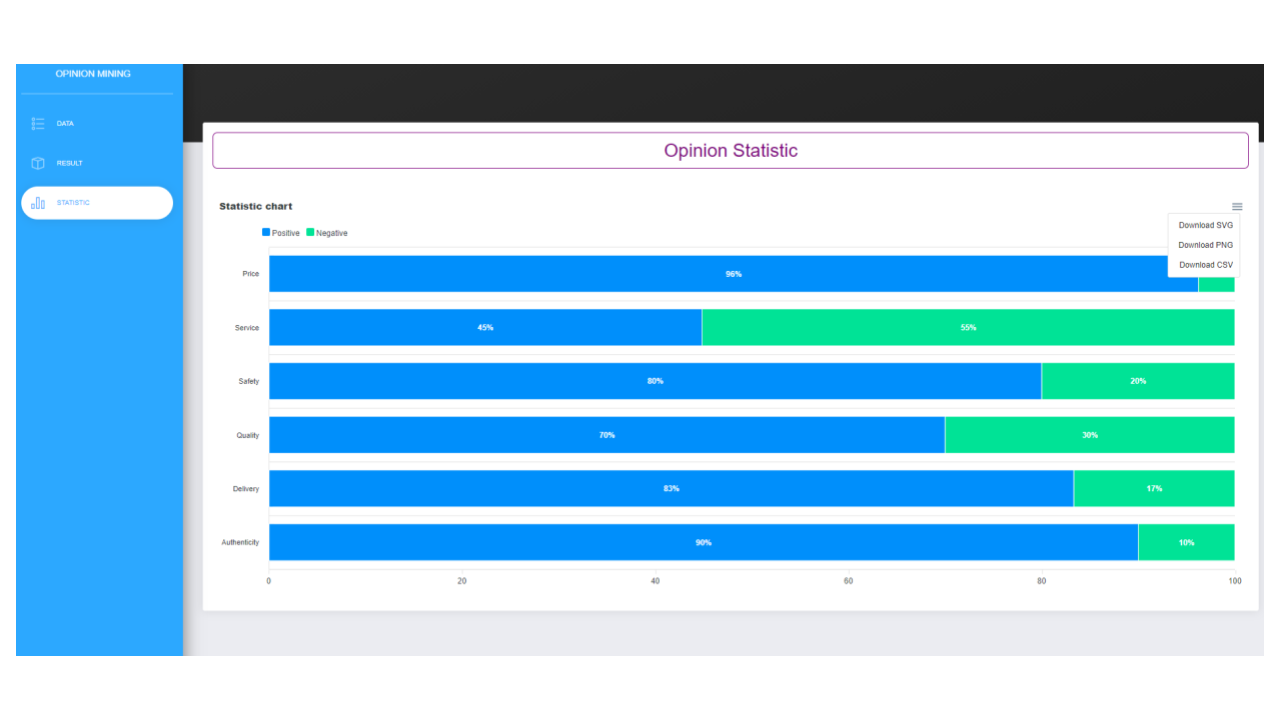
\includegraphics[width=\linewidth]{Chapter4/Figs/tool5.png}
	\caption{Detailed statistical results of positive and negative sentiment on each aspects}
	\label{fig:tool5}
\end{figure}

\chapter{Conclusions}
\addcontentsline{toc}{chapter}{Conclusions}
\label{chap:conclusion}

% -------------------------------------------------------------------
% Contributions
% -------------------------------------------------------------------
\section*{Contributions}
In this article, we proposed multiple approaches for the sentiment polarity detection - a sub-task of ABSA problem. Experiments indicated significant result as WWL combine with classic models has reach the maximum percentage of 95\% in Micro- and Macro-Average Performance of F1-score.

% -------------------------------------------------------------------
% Results
% -------------------------------------------------------------------
Through experiments using the locating method and apply multiple data representation techniques, we can determine that using the WWL method with the Chi-Squared data representation brings very prominent results when combined with traditional machine learning methods. Because when classify the sentiment for multi-label data (i.e., multiple aspects in a data sample) using multiple models, we need to find the words associated with the label and the word representing its sentiment. WWL technique step solves this problem. In addition, in order for the data to focus on important words, we use Chi-Squared score to weight word level in the vocab and use it to represent data. This combination brings the most outstanding advantage to address the problem.

% -------------------------------------------------------------------
% Limitations and Future Work
% -------------------------------------------------------------------
\section*{Limitations and Future Work}
Selecting threshold for locating words inappropriately may be harmful to the result of the model. Window size (i.e., the number of words around from the center, which equals 3 in the proposed work) affects final result too. This requires manual data revision to be done carefully to choose which one is the best. This is the limitation of our method.

The weak point of proposed work indicates our next path to have in-depth research in the future: 

(i) More data should be collected to enlarge the dataset.

(ii) Handling the data imbalance problem.

(iii) Developing WWL in order to overcome current disadvantage.
% We released our source code and data on the public repository to support the re-producibility of our work and facilitate other related studies.

% \include{Chapter6/chapter6}


% % List of publications
% \chapter*{List of Publications}
\addcontentsline{toc}{chapter}{List of Publications}

\begin{enumerate}[label={[Pub \arabic*]},leftmargin=3cm]

\item \underline{\textbf{Duy-Cat Can}}, Hoang-Quynh Le, Quang-Thuy Ha, and Nigel Collier. ``A Richer-but-Smarter Shortest Dependency Path with Attentive Augmentation for Relation Extraction.'' In \textit{The 2019 Annual Conference of the North American Chapter of the Association for Computational Linguistics: Human Language Technologies (NAACL-HTL)}, 2019, (In Press).

\item \underline{\textbf{Duy-Cat Can}}, Hoang-Quynh Le, and Quang-Thuy Ha. ``Improving Semantic Relation Extraction System with Compositional Dependency Unit on Enriched Shortest Dependency Path.'' In \textit{The 11th Asian Conference on Intelligent Information and Database Systems (ACIIDS)}, pp. 140-152, Springer, 2019.

\item Trang M. Nguyen, Van-Lien Tran, \underline{\textbf{Duy-Cat Can}}, Quang-Thuy Ha, Ly T. Vu, and Eng-Siong Chng. ``QASA: Advanced Document Retriever for Open-Domain Question Answering by Learning to Rank Question-Aware Self-Attentive Document Representations.'' In \textit{Proceedings of the 3rd International Conference on Machine Learning and Soft Computing}, pp. 221-225. ACM, 2019.

\item \underline{\textbf{Duy-Cat Can}}, Thi-Nga Ho, and Eng-Siong Chng. ``A hybrid deep learning architecture for sentence unit detection.'' In \textit{Proceedings of the 2018 International Conference on Asian Language Processing (IALP)}, pp. 129-132. IEEE, 2018.

\item Thi-Nga Ho, \underline{\textbf{Duy-Cat Can}}, and Eng-Siong Chng. ``An investigation of word embeddings with deep bidirectional lstm for sentence unit detection in automatic speech transcription.'' In \textit{Proceedings of the International Conference on Asian Language Processing (IALP)}, pp. 139-142. IEEE, 2018.

\item Hoang-Quynh Le, \underline{\textbf{Duy-Cat Can}}, Sinh T. Vu, Thanh Hai Dang, Mohammad Taher Pilehvar, and Nigel Collier. ``Large-scale exploration of neural relation classification architectures.'' In \textit{Proceedings of the 2018 Conference on Empirical Methods in Natural Language Processing (EMNLP)}, pp. 2266-2277. 2018.

\end{enumerate}

%--------------------------------------------- 
% References
%---------------------------------------------
\bibliographystyle{IEEEtranSN}
\renewcommand\bibname{References}
\addcontentsline{toc}{chapter}{References}
\bibliography{references} % Path to your references.bib file

%--------------------------------------------- 
% Appendix
%---------------------------------------------
\appendix
% \chapter{List of Publications}
Appendix A

\end{document}
